\documentclass[12pt]{article}
\usepackage{graphicx}
\usepackage{spverbatim}
\usepackage{listings}
\usepackage[T1]{fontenc}
\usepackage{geometry}
\geometry{letterpaper, margin=0.75in}

\input{pygments.tex}

\begin{document}

\title{CS472 Assignment 3}
\author{Mark Bereza}
\date{\today}
\maketitle

\section*{Part 1}
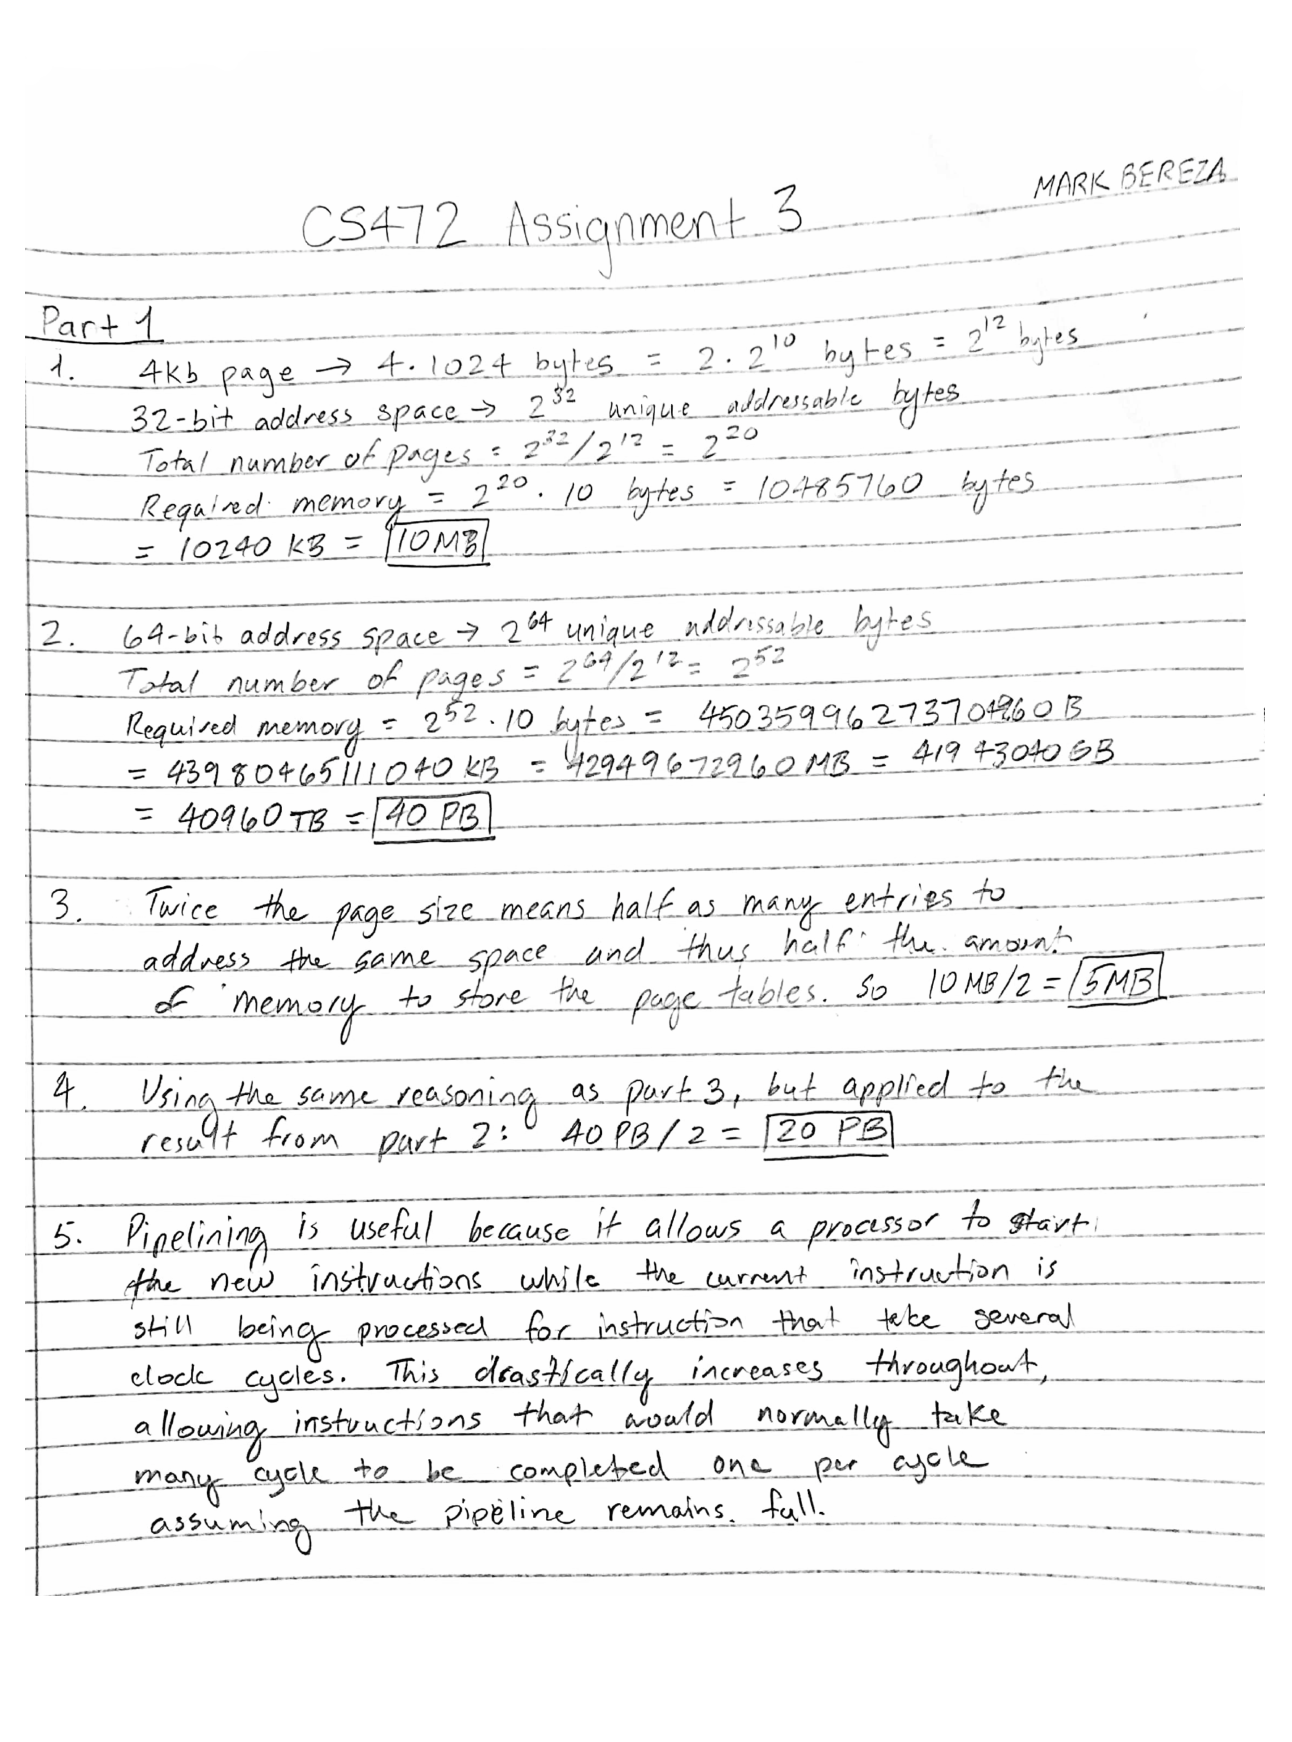
\includegraphics[width=\textwidth]{part11.eps}
\clearpage
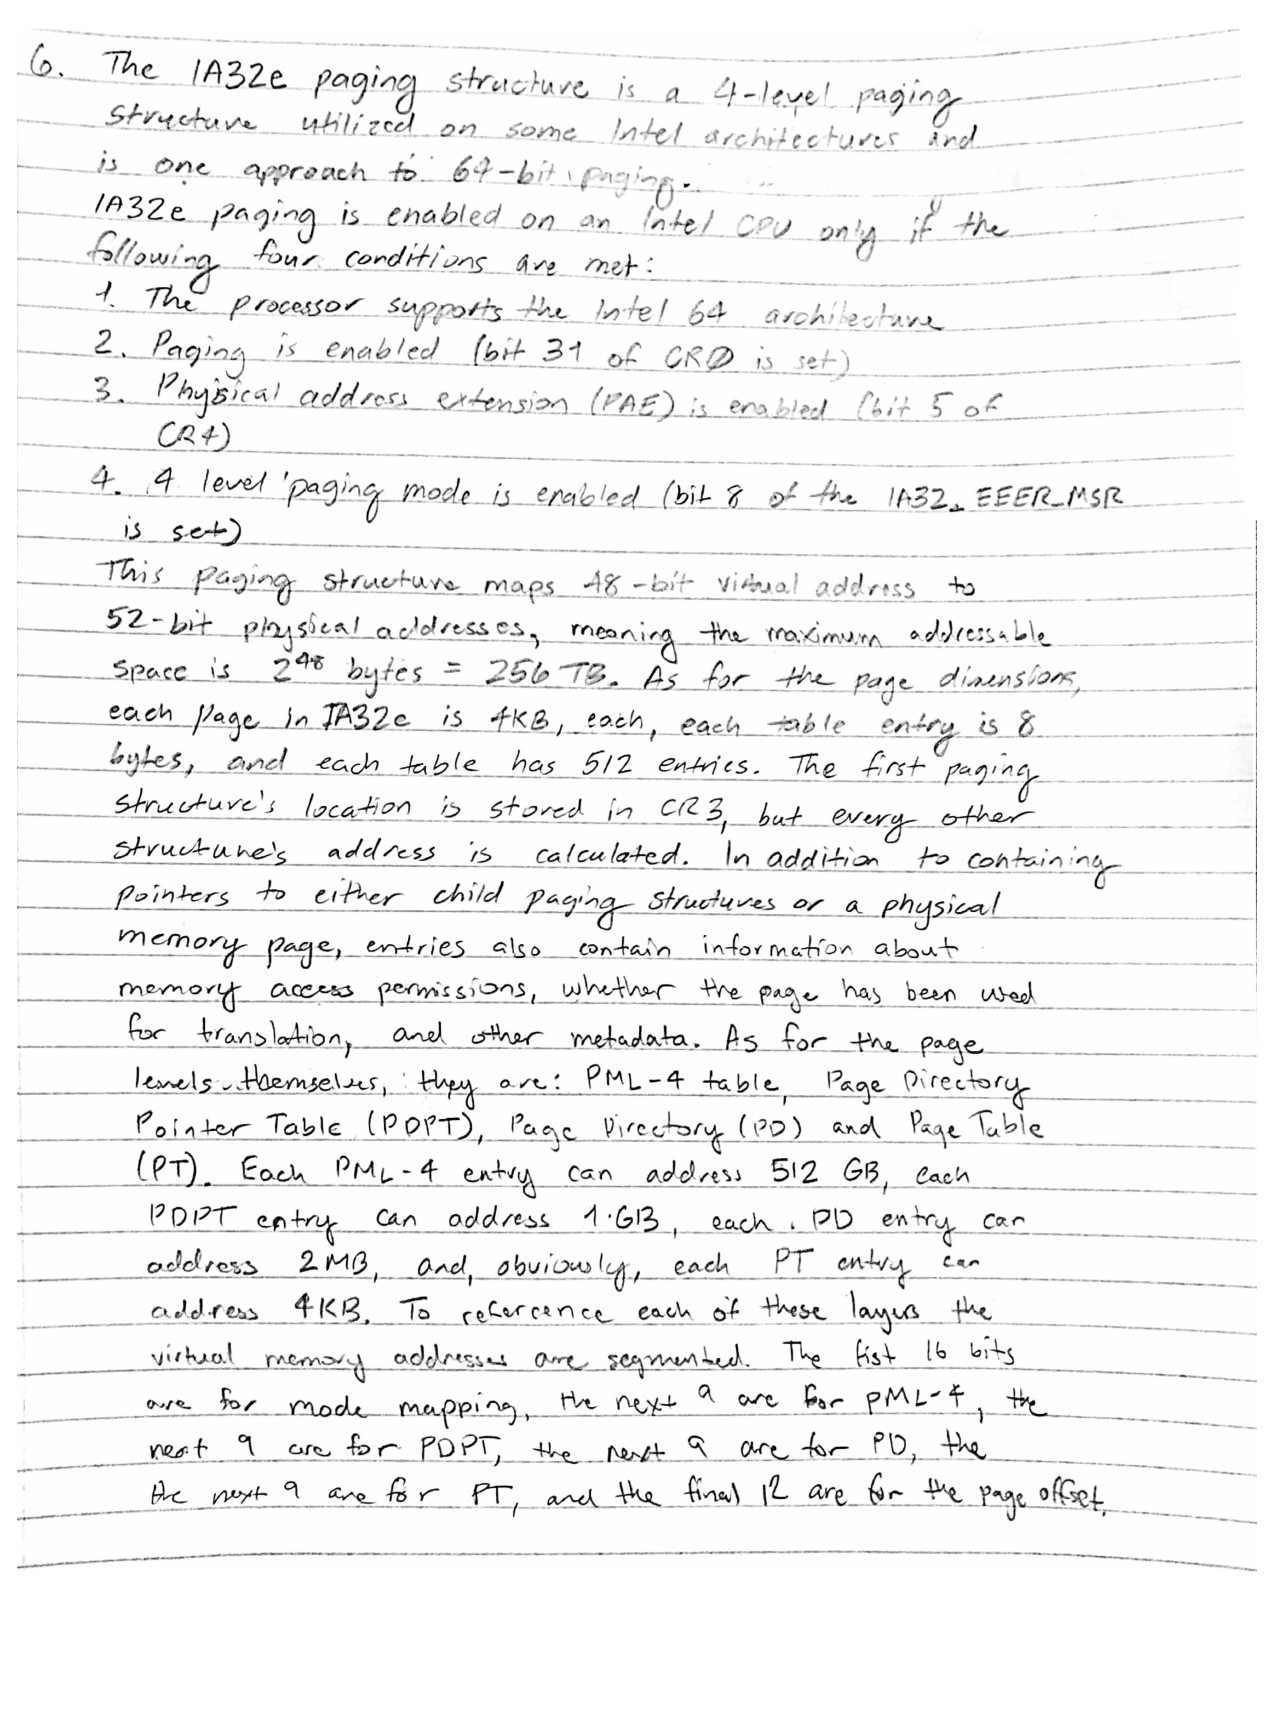
\includegraphics[width=\textwidth]{part12.eps}
\clearpage
\section*{Part 2}
\subsection*{"Memory Optimization" Summary}
This presentation makes an argument for why memory optimization is something programmers should be aware of and try to attain in their code. The author claims that the reasons why it is important for programmers to write cache-aware code are that memory access speeds have increased slowly compared to CPU clock speeds, the cache is generally under utilized, and compilers are generally poor at figuring out how to optimize memory accessing on their own.

The author then describes the various reasons why caches might "miss" and goes into detail describing strategies to improve one's code to reduce these misses and increases performance overall by making better use of the cache. These strategies include profiling one's code to get a better picture of when and where memory accesses are occuring, reordering code to improve locality, and compressing/padding code to improve use of cache lines. In particular, the presentation touches upon prefetching/preloading data that will be used in an anticipatory fashion, reordering fields in structures/objects based on actual use and hot vs cold members, and cache-aware approaches to tree-like data structures. The author further suggests the use of memory pools and linearization of hierchial data to increase spatial locality and thus incrases cache hit rate. Finally, the author discusses the cache performance penalties associated with aliasing (multiple indirect references to the same memory location) and higher levels of abstraction, which both make it harder for the compiler to optimize read accesses. The rest of the presentation is devoted to detailing several strategies for minimizing aliasing, including consuming pointer variables into distinct local variables, avoiding class abstraction where possible, making variables of incompatible types explicitly so to the compiler, and leveraging C's 'restrict' keyword. 
\subsection*{"What Every Programmer Should Know About Memory" Summary}
Our interest in this paper has to do with computation of cache sizes. First, in section 3.3.1, the paper states that the total cache size may computed using the following formula:\\ \\
\begin{center}
$\textrm{cache size} = \textrm{cache line size} \cdot \textrm{associativity} \cdot \textrm{number of sets}$
\end{center}
\par Beyond that, section 6.2.3 describes how to compute a safe lower limit for cache size on a Linux machine. This involves reading\\ \spverb|/sys/devices/system/cpu/cpu*/cache/size| and dividing ``the numeric value contained within by the number of bits set in the file \verb!shared_cpu_map!." 
\par Alternatively, an easier method presented in the paper involves calling \verb!sysconf()! with a macro defining the cache to be queried passed as its only argument.
\section*{Part 3}
For this part, I simply inspected the contents of the files located under /sys/devices/system/cpu/cpu0/cache/ to determine the number of caches, their level, their type, their line size, their number of sets, and their ways of association. Here, I made the assumption that these properties would be the same across the different cores and thus querying a single core's data would be sufficient. 
\subsection*{Source Code}
\input{__part3.c.tex}
\section*{Part 4}
For this part, I simply wrote a function that would reverse the order of bytes for any byte array. Then, I used a preprocessor directive to determine the endianness of the system. If the system was determined to be little-endian, byte swapping was performed. Otherwise, the data was left as-is.
\subsection*{Source Code}
\input{__part4.c.tex}
\section*{Part 5}
For this part, I change the \verb!byte_swap()! function to first determine the endianness of the system at runtime by storing \verb!0x0102! to the integer portion of a union and checking whether the first byte (via array indexing) was 1 or 2. If the first byte was 1, then the system was big-endian. Otherwise, it was little-endian. As with Part 4, byte swapping was performed if the system was determined to be little-endian.
\subsection*{Source Code}
\input{__part5.c.tex}
\end{document}
